\documentclass[border=2mm]{standalone}

\usepackage{fontspec}
\usepackage{unicode-math}
\usepackage{amsmath}

\usepackage{pgfplots}
\pgfplotsset{compat=1.18}
\usetikzlibrary{arrows.meta, 
  calc, 
  positioning, 
  decorations.pathreplacing, 
  calligraphy}
\usetikzlibrary{patterns}

\usepackage{xcolor}
\definecolor{den-1}{HTML}{111111}   % Đen #111111
\definecolor{den-2}{HTML}{222222}   % Đen #222222
\definecolor{den-3}{HTML}{333333}   % Đen #333333
\definecolor{den-4}{HTML}{444444}   % Đen #444444
\definecolor{den-5}{HTML}{555555}   % Đen #555555
\definecolor{den-6}{HTML}{666666}   % Đen #666666


\begin{document}

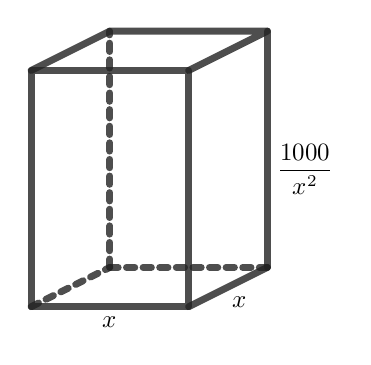
\begin{tikzpicture}[scale=1, line cap=round, line join=round]

  \draw [line width=2.5pt, color=den-2, opacity=.8] 
    (0,0) -- (2,0) -- (2,3) -- (0,3) -- cycle;
  \draw [dashed, line width=2.5pt, color=den-2, opacity=.8] 
    (0,0) -- (1,.5);
  \draw [dashed, line width=2.5pt, color=den-2, opacity=.8] 
    (1,.5) -- (3,.5);
  \draw [line width=2.5pt, color=den-2, opacity=.8] 
    (3,.5) -- (2,0);
  \draw [line width=2.5pt, color=den-2, opacity=.8] 
    (0,3) -- (1,3.5) -- (3,3.5) -- (2,3);
  \draw [dashed, line width=2.5pt, color=den-2, opacity=.8] 
    (1,.5) -- (1,3.5);
  \draw [line width=2.5pt, color=den-2, opacity=.8] 
    (3,.5) -- (3,3.5);

  % Nhãn
  \node at (1,0) [below] {\small $x$};
  \node at (2.65,.25) [below] {\small $x$};
  \node at (3,1.75) [right] {\small $\dfrac{1000}{x^2}$};

\end{tikzpicture}


\end{document}
